% LectureTemplate for ME3050 -  Dynamics Modeling and Controls - Tennessee Technological University
% Tristan Hill - Spring 2020 - Summer 2020 - Fall 2022
% Dynamics Modeling and Controls
% Lecture Module - Introduction - Topic 3 - Modeling Assumptions

% Document settings

%\documentclass{beamer}                  % for presentation ?
\documentclass[handout]{beamer}  % for handout ?

\usepackage{/home/thill/Documents/lectures/dmc_lectures/dmc_lectures}

\newcommand{\MNUM}{1\hspace{2mm}} % Module number
\newcommand{\TNUM}{3\hspace{2mm}} % Topic number 
\newcommand{\moduletitle}{Introduction} % Titles and Stuff
\newcommand{\topictitle}{Modeling Assumptions} 

\newcommand{\sectiontitleI}{Simplify Complex Systems} % More Titles and Stuff
\newcommand{\sectiontitleII}{Increase Complexity Incrementally}
\newcommand{\sectiontitleIII}{Solid Mechanics and Dynamics}
\newcommand{\sectiontitleIV}{Thermal and Fluid Systems}
\newcommand{\sectiontitleV}{Electrical and Power Systems}


\author{ME3050 - Dynamic Modeling and Controls}
\title{Module \MNUM - \moduletitle}
\date{Mechanical Engineering\vspc Tennessee Technological University}

\begin{document}

\lstset{language=MATLAB,basicstyle=\ttfamily\small,showstringspaces=false}

\frame{\titlepage \center\begin{framed}\Large \textbf{Topic \TNUM - \topictitle}\end{framed} \vspace{5mm}}

% Section 0 - Outline
\frame{
	
	\large \textbf{Topic \TNUM - \topictitle} \vspace{3mm}\\
	
	\begin{itemize}
	
		\item \sectiontitleI    \vspc % Section I
		\item \sectiontitleII 	\vspc % Section II
		\item \sectiontitleIII 	\vspc %Section III
		\item \sectiontitleIV 	\vspc %Section IV
		\item \sectiontitleV 	\vspc %Section V
	
	\end{itemize}

}

% Section 1:
\section{Simplify Complex Systems}

\frame{
\frametitle{Simplify Complex Systems}
\begin{multicols}{2}
Engineers encounter complex systems and these systems are difficult to model and analyze.  Analysis requires multiple steps or processes and modeling requires iteration. Typically, you cannot solve these complex problems in your head alone. \vspc

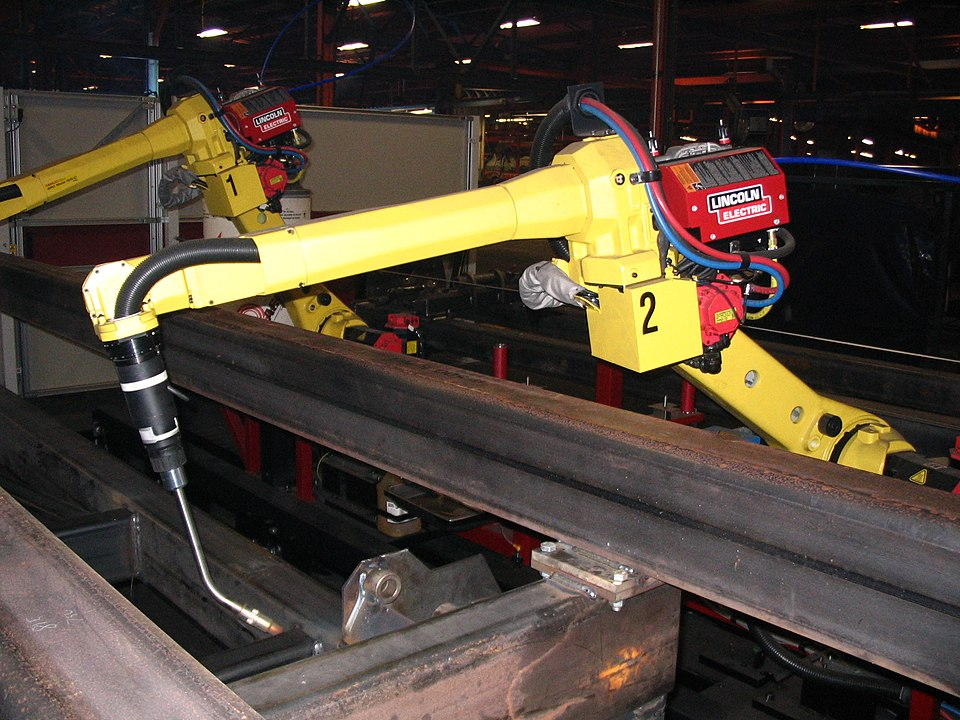
\includegraphics[scale=.15]{fanuc_robot.jpg}
\end{multicols}
{\tiny \hspace{60mm} Image: \href{https://en.wikipedia.org/wiki/Articulated_robot}{Wikipedia} }

}

% Section 2: 
\section{Increase Complexity Incrementally}

\frame{
\frametitle{Increase Complexity Incrementally}


Engineers model and analyze complex systems one piece at a time on a component level. \vspc

In system dynamics we study the behavior of complex systems by modeling the iterations and responses of the different components involved. Our models will start simple and build in complexity as the theory is presented. 

}

% Section 3: 
\section{Solid Mechanics and Dynamics}

\frame{
\frametitle{Solid Mechanics and Dynamics}

\begin{multicols}{2}
\begin{itemize}
\item Frictionless Sliding  ?
\item Pure Roll - No Slip 
\item Planar Motion \\
\end{itemize}

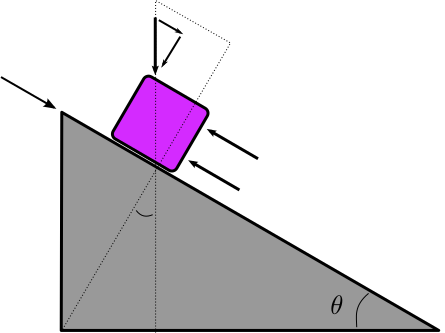
\includegraphics[scale=0.209]{sliding_block.png}
 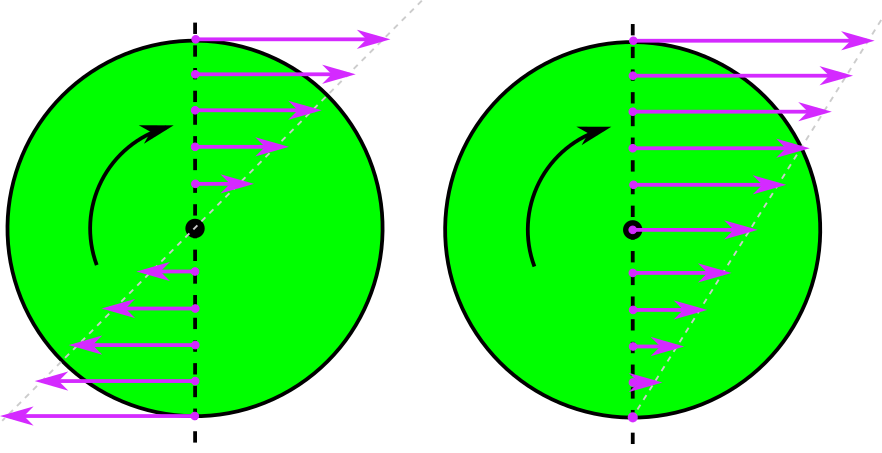
\includegraphics[scale=0.125]{pure_roll_no_slip.png} 
 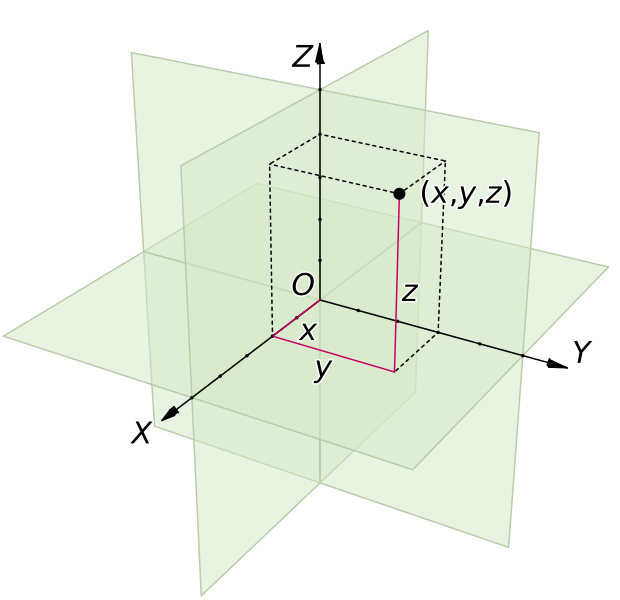
\includegraphics[scale=0.17]{cartesian_3d.png}
\end{multicols}
{\tiny Image: TH\hspace{60mm} Images: TH, \href{https://en.wikipedia.org/wiki/Cartesian_coordinate_system}{Wikipedia} }

}

% Section 4:
\section{Thermal and Fluid Systems}

\frame{
\frametitle{Thermal and Fluid Systems}

\begin{itemize}
\item Viscous Boundary Layer
\item Insulated or Constant Flux Boundaries
\item Others?
\end{itemize}

}

% Section 5:
\section{Electrical and Power Systems}

\frame{
\frametitle{Electrical and Power Systems}

\begin{multicols}{2}
\begin{itemize}
\item No Heat Loss or Generation
\item Ideal Conductors
\item Zero Order, First Order System Behavior
\end{itemize}

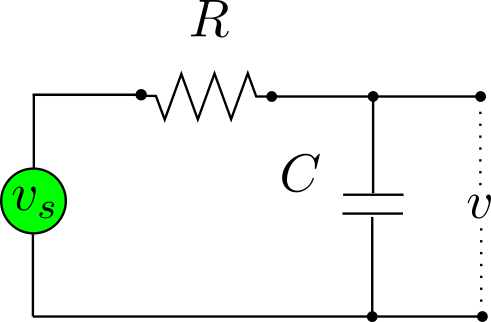
\includegraphics[scale=.25]{rc_circuit.png}
\end{multicols}
{\hspace{60mm}\tiny Image: TH}
}
	
\end{document}



